\chapter{System overview}\label{cha:overview}

In this chapter an description of the system is made. This is made for the reader to get a better understanding of the setup which was available at Aalborg university. This description includes the following points and will be described in the same order, then a system overview is provided.

\begin{itemize}
  \item The Geomagic Touch,
  \item The da Vinci robot,
  \item The EndoWrist,
  \item The electronics,
  \item The mechanical test setup
\end{itemize}
\todo{update itemizer later so it fits!}

\section{Da vinci robot}\label{sec:da_vin_rob}

The Da vinci robot is a minimal invasive surgery (MSI) robot used in surgeries such as cardiac, coloretal and gynecologic surgeries\cite{daVinciSurgery}. The version available on Aalborg university is the first generation, see \figref{fig:fulldavinci}.

\begin{figure}[H]
	\centering
	\begin{subfigure}{.45\textwidth}
		\centering
		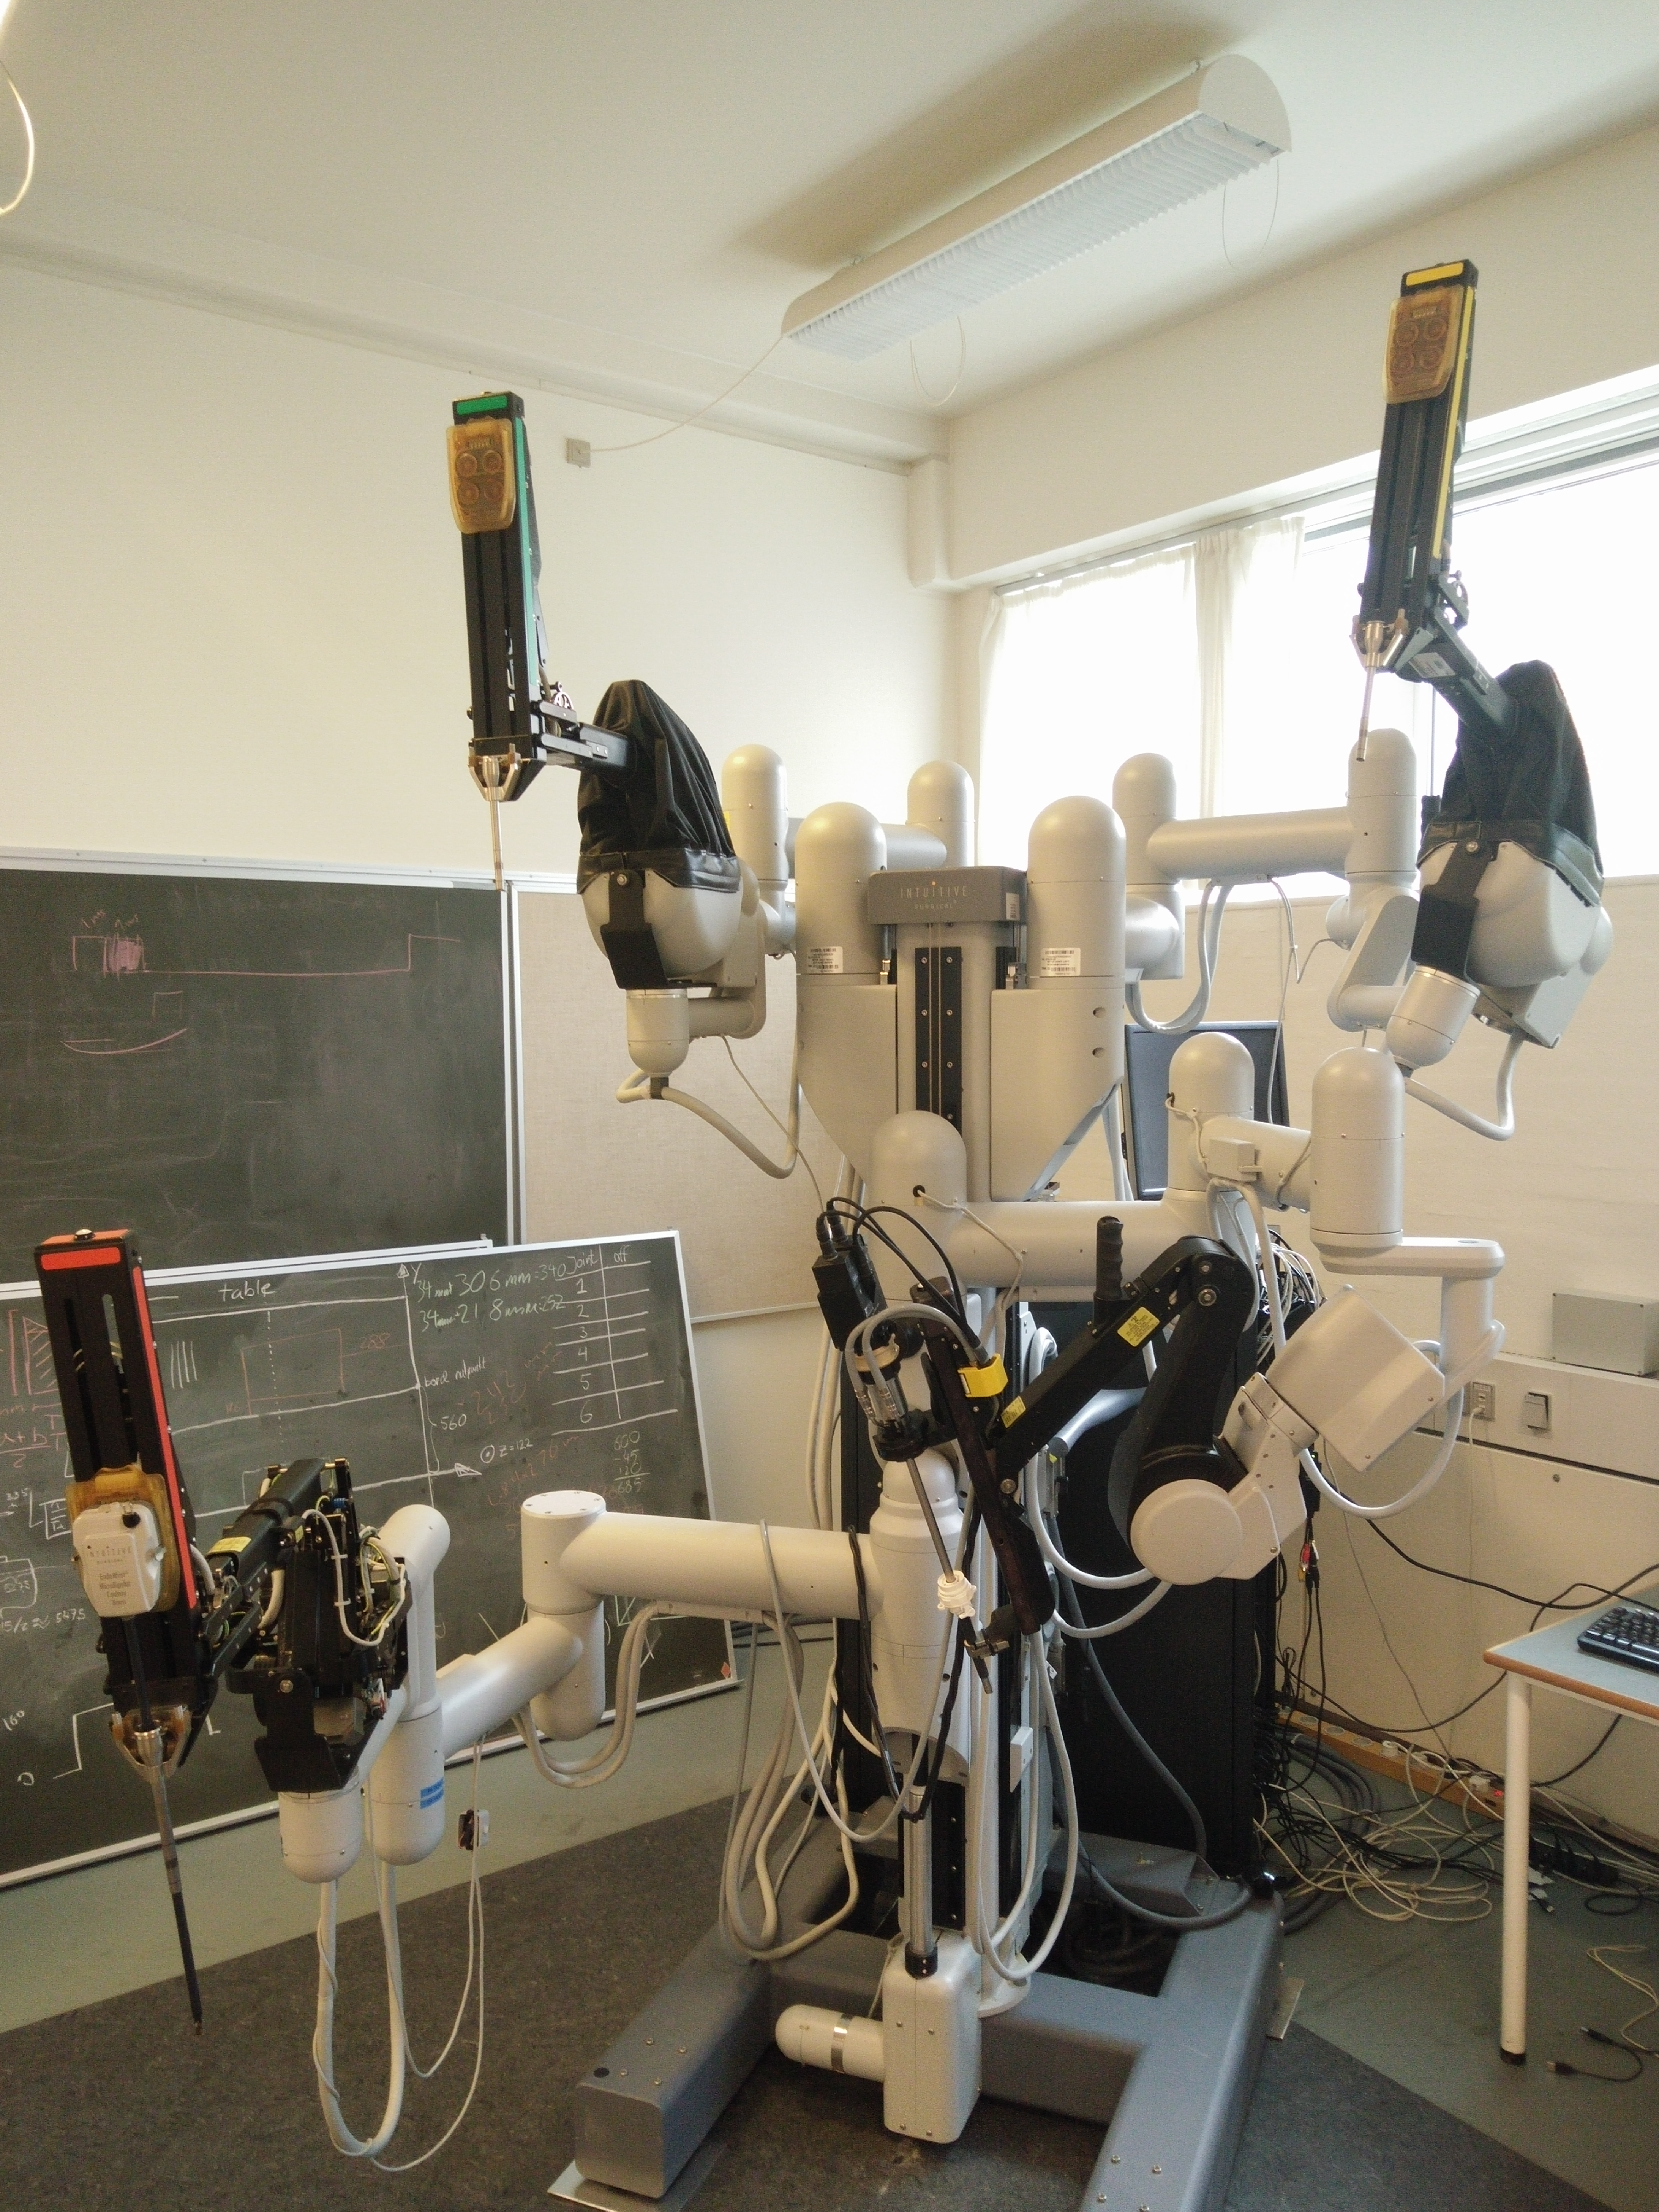
\includegraphics[width=\linewidth]{DavinciRobot.jpg}
		\caption{The da vinci robot or slave manipulator.}
		\label{fig:davincirobot}
	\end{subfigure}
	\begin{subfigure}{.45\textwidth}
		\centering
		\vspace{12pt}
		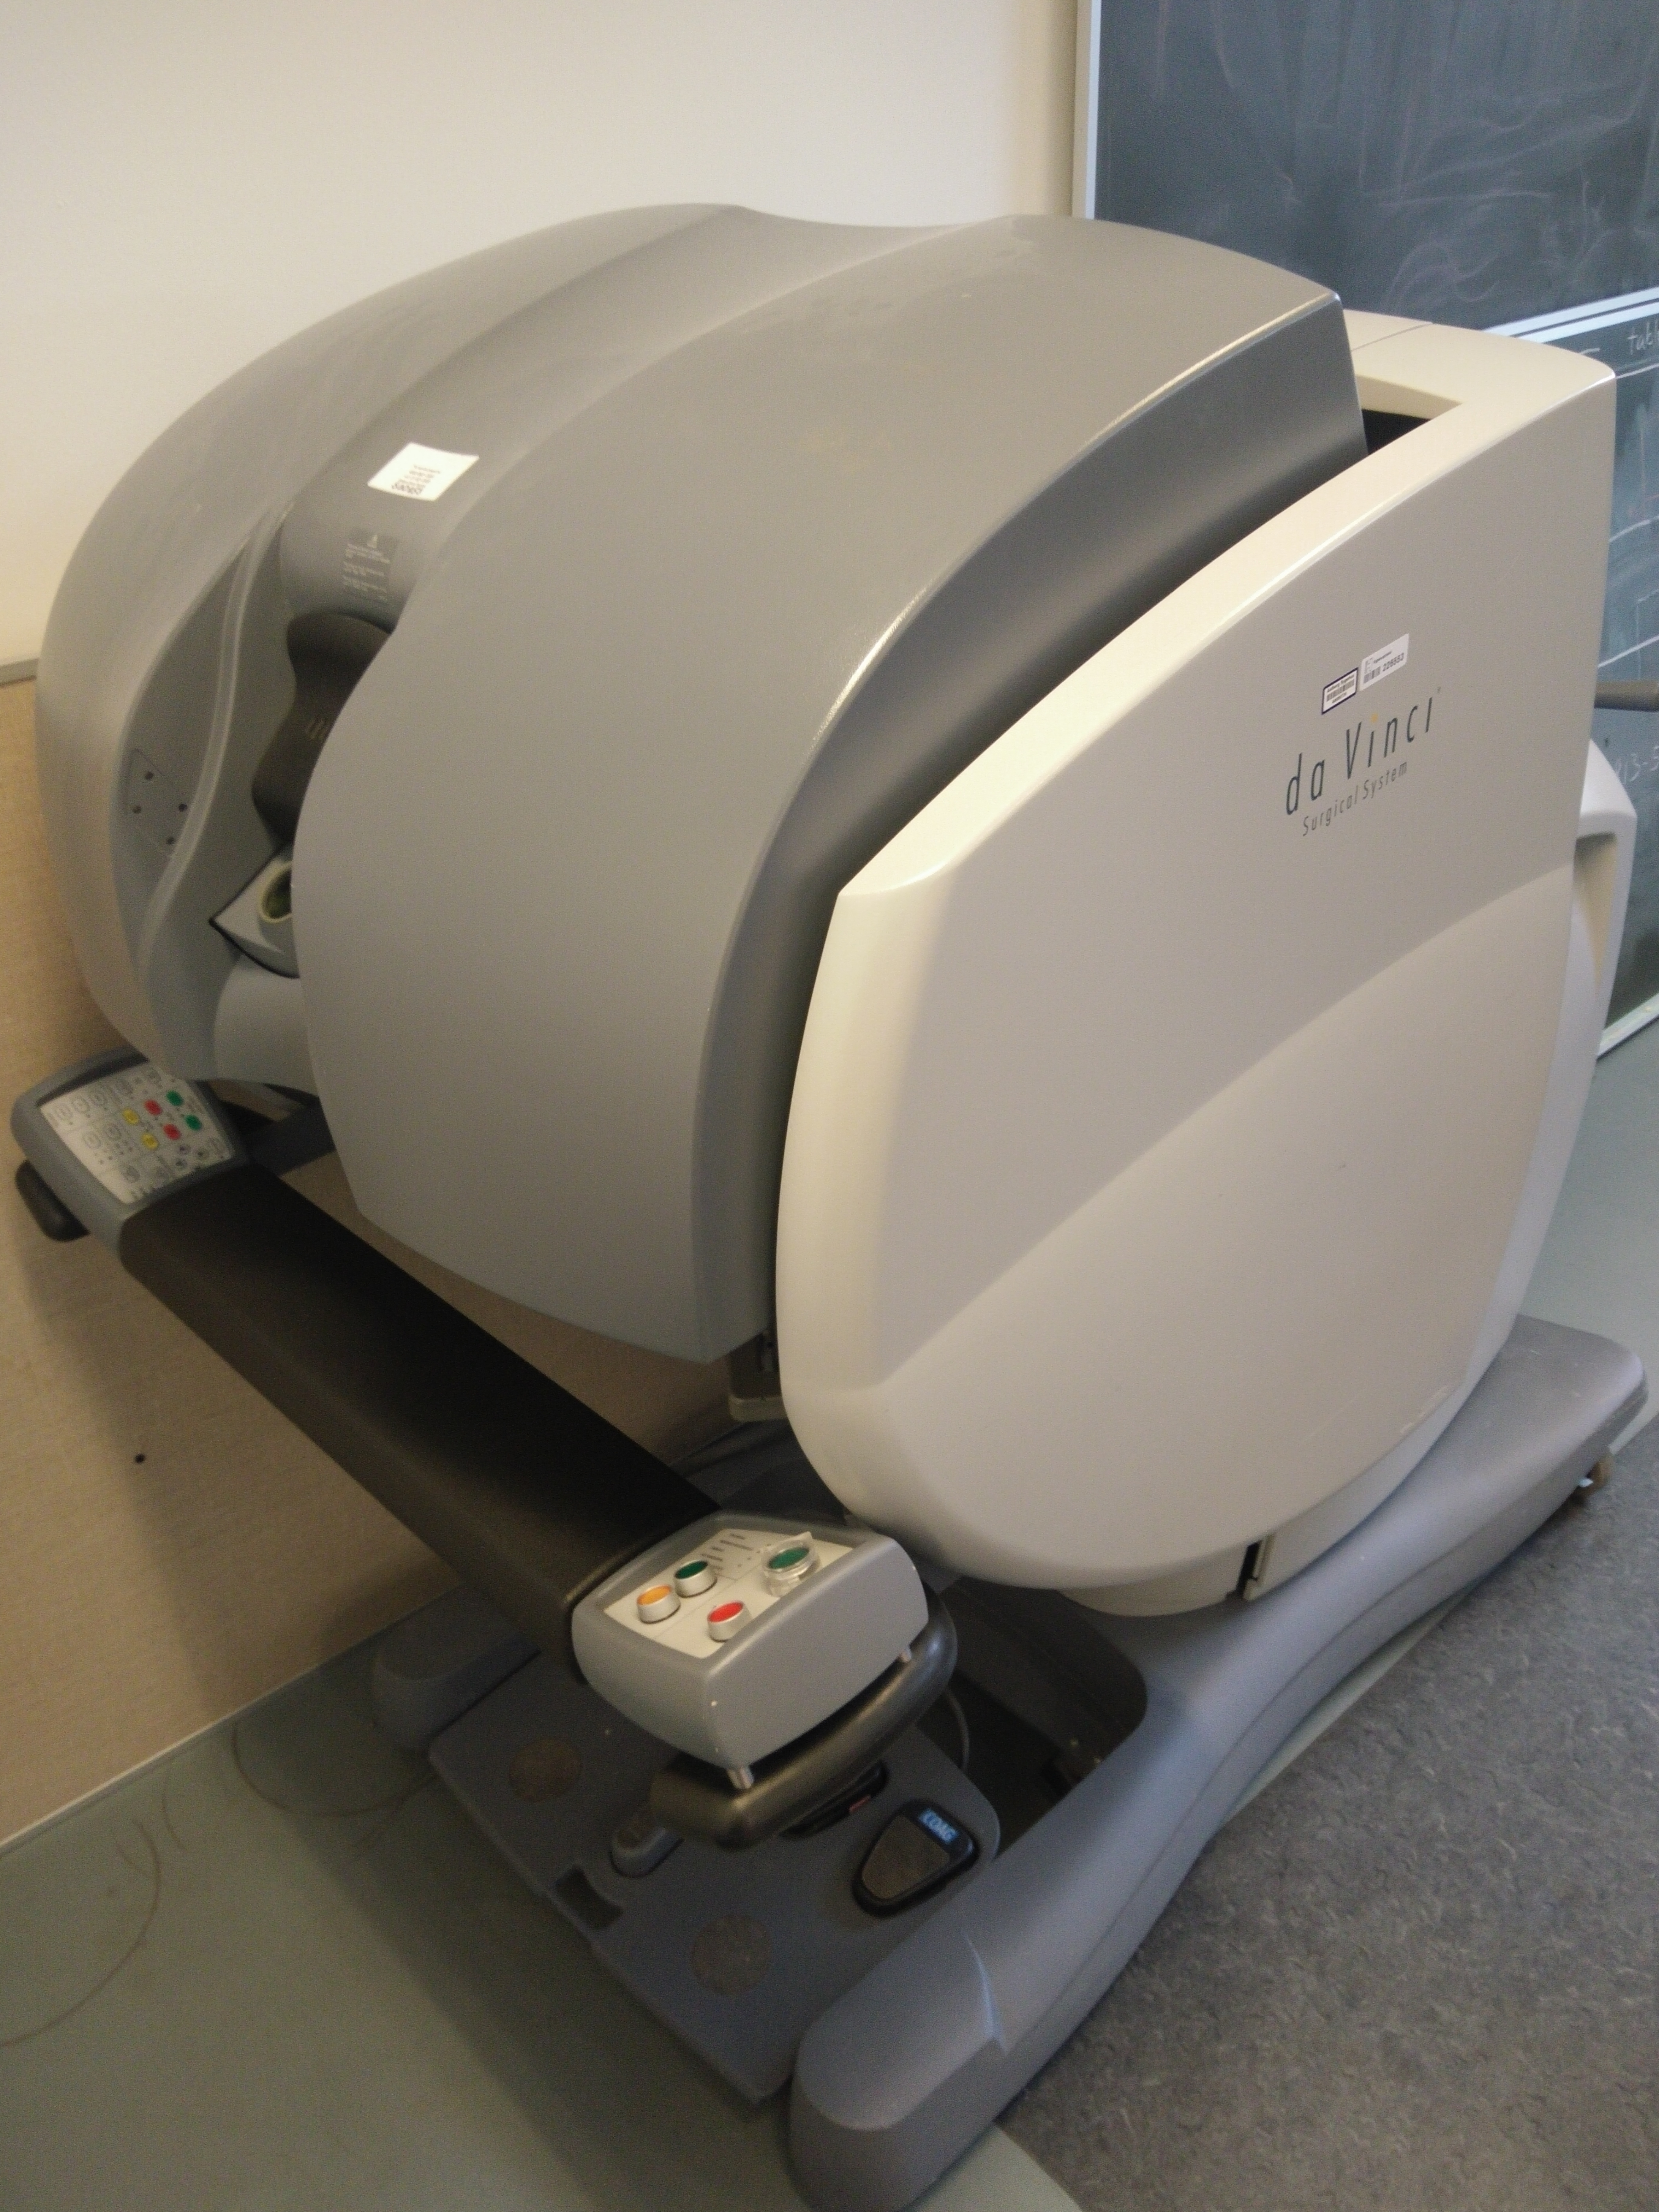
\includegraphics[width=\linewidth]{masterconsole.jpg}
		\caption{The master console to control the slave manipulator.}
		\label{fig:mastermani}
	\end{subfigure}
\caption{Full view of the Da vinci surgery system which include the slave manipulator and the master console}
\label{fig:fulldavinci}
\end{figure}

It consists of two main parts, a master console, see \figref{fig:mastermani}, and a slave manipulator, see \figref{fig:davincirobot}.

\begin{itemize}
\item The surgeon uses the master console to control the slave manipulator. It consists of two eye pieces, which display a high resolution 3D view of the surgery for the surgeon. 
\item The slave manipulator is the robot which is controlled by the master console by the surgeon. It consists of four arms with 6-7 \gls{DOF} each, depending on the end.
\end{itemize}

The master console and three of the slave manipulators arms are disabled from the system. The console is disabled from the system, since force feedback is not an option on this device. The three arms are disabled since the control on these will be identical. The master console will not be further analyzed. To control the last arm on the slave manipulator, the Geomagic touch, see \secref{sec:geo_magic}, has been implemented as the master controller.

%a replacement master controller called a Geo magic touch is implemented, see \secref{sec:geo_magic}.


\subsection*{Slave manipulator arm}
The slave manipulator arm consists of of three parts, arm, hand and tool, see \figref{fig:davinciarmrobot}.

\begin{figure}[H]
	\centering
		\centering
		\includegraphics[width=0.85\linewidth]{davincirobotarm_label.jpg}
		\caption{One extended arm of the da vinci robot, where the arm, hand and EndoWrist/tool are defined.}
		\label{fig:davinciarmrobot}
\end{figure}


\begin{enumerate}
\item Arm:

The arm of the tool is the part which is furtherest away from the patient. 
Under surgery it is locked to a specific position. Therefore it is not possible to change its position during the operation.
\item Hand

The hand is at the end of the arm and has three \gls{DOF}, which can be actuated under surgery.
\item Tool / end effector 

The tool is connected to the hand. Together these got 6 - 7 movable \gls{DOF} that can be actuated. The tool is the instrument which interacts with the patient under surgery. There are several different tools available, each with their own functionality. 
\end{enumerate}



\section{Geomagic touch}\label{sec:geo_magic}
The geomagic touch is a haptic feedback device, which has the ability to manipulates its joint in such a way that the user feels resistance when moving the pin in a certain direction or way. The geomagic touch described in this section is the model Phantom omni and can be seen on \figref{fig:phantom_omni}.

\begin{figure}[H]
	\centering
	\begin{subfigure}{.45\textwidth}
		\centering
		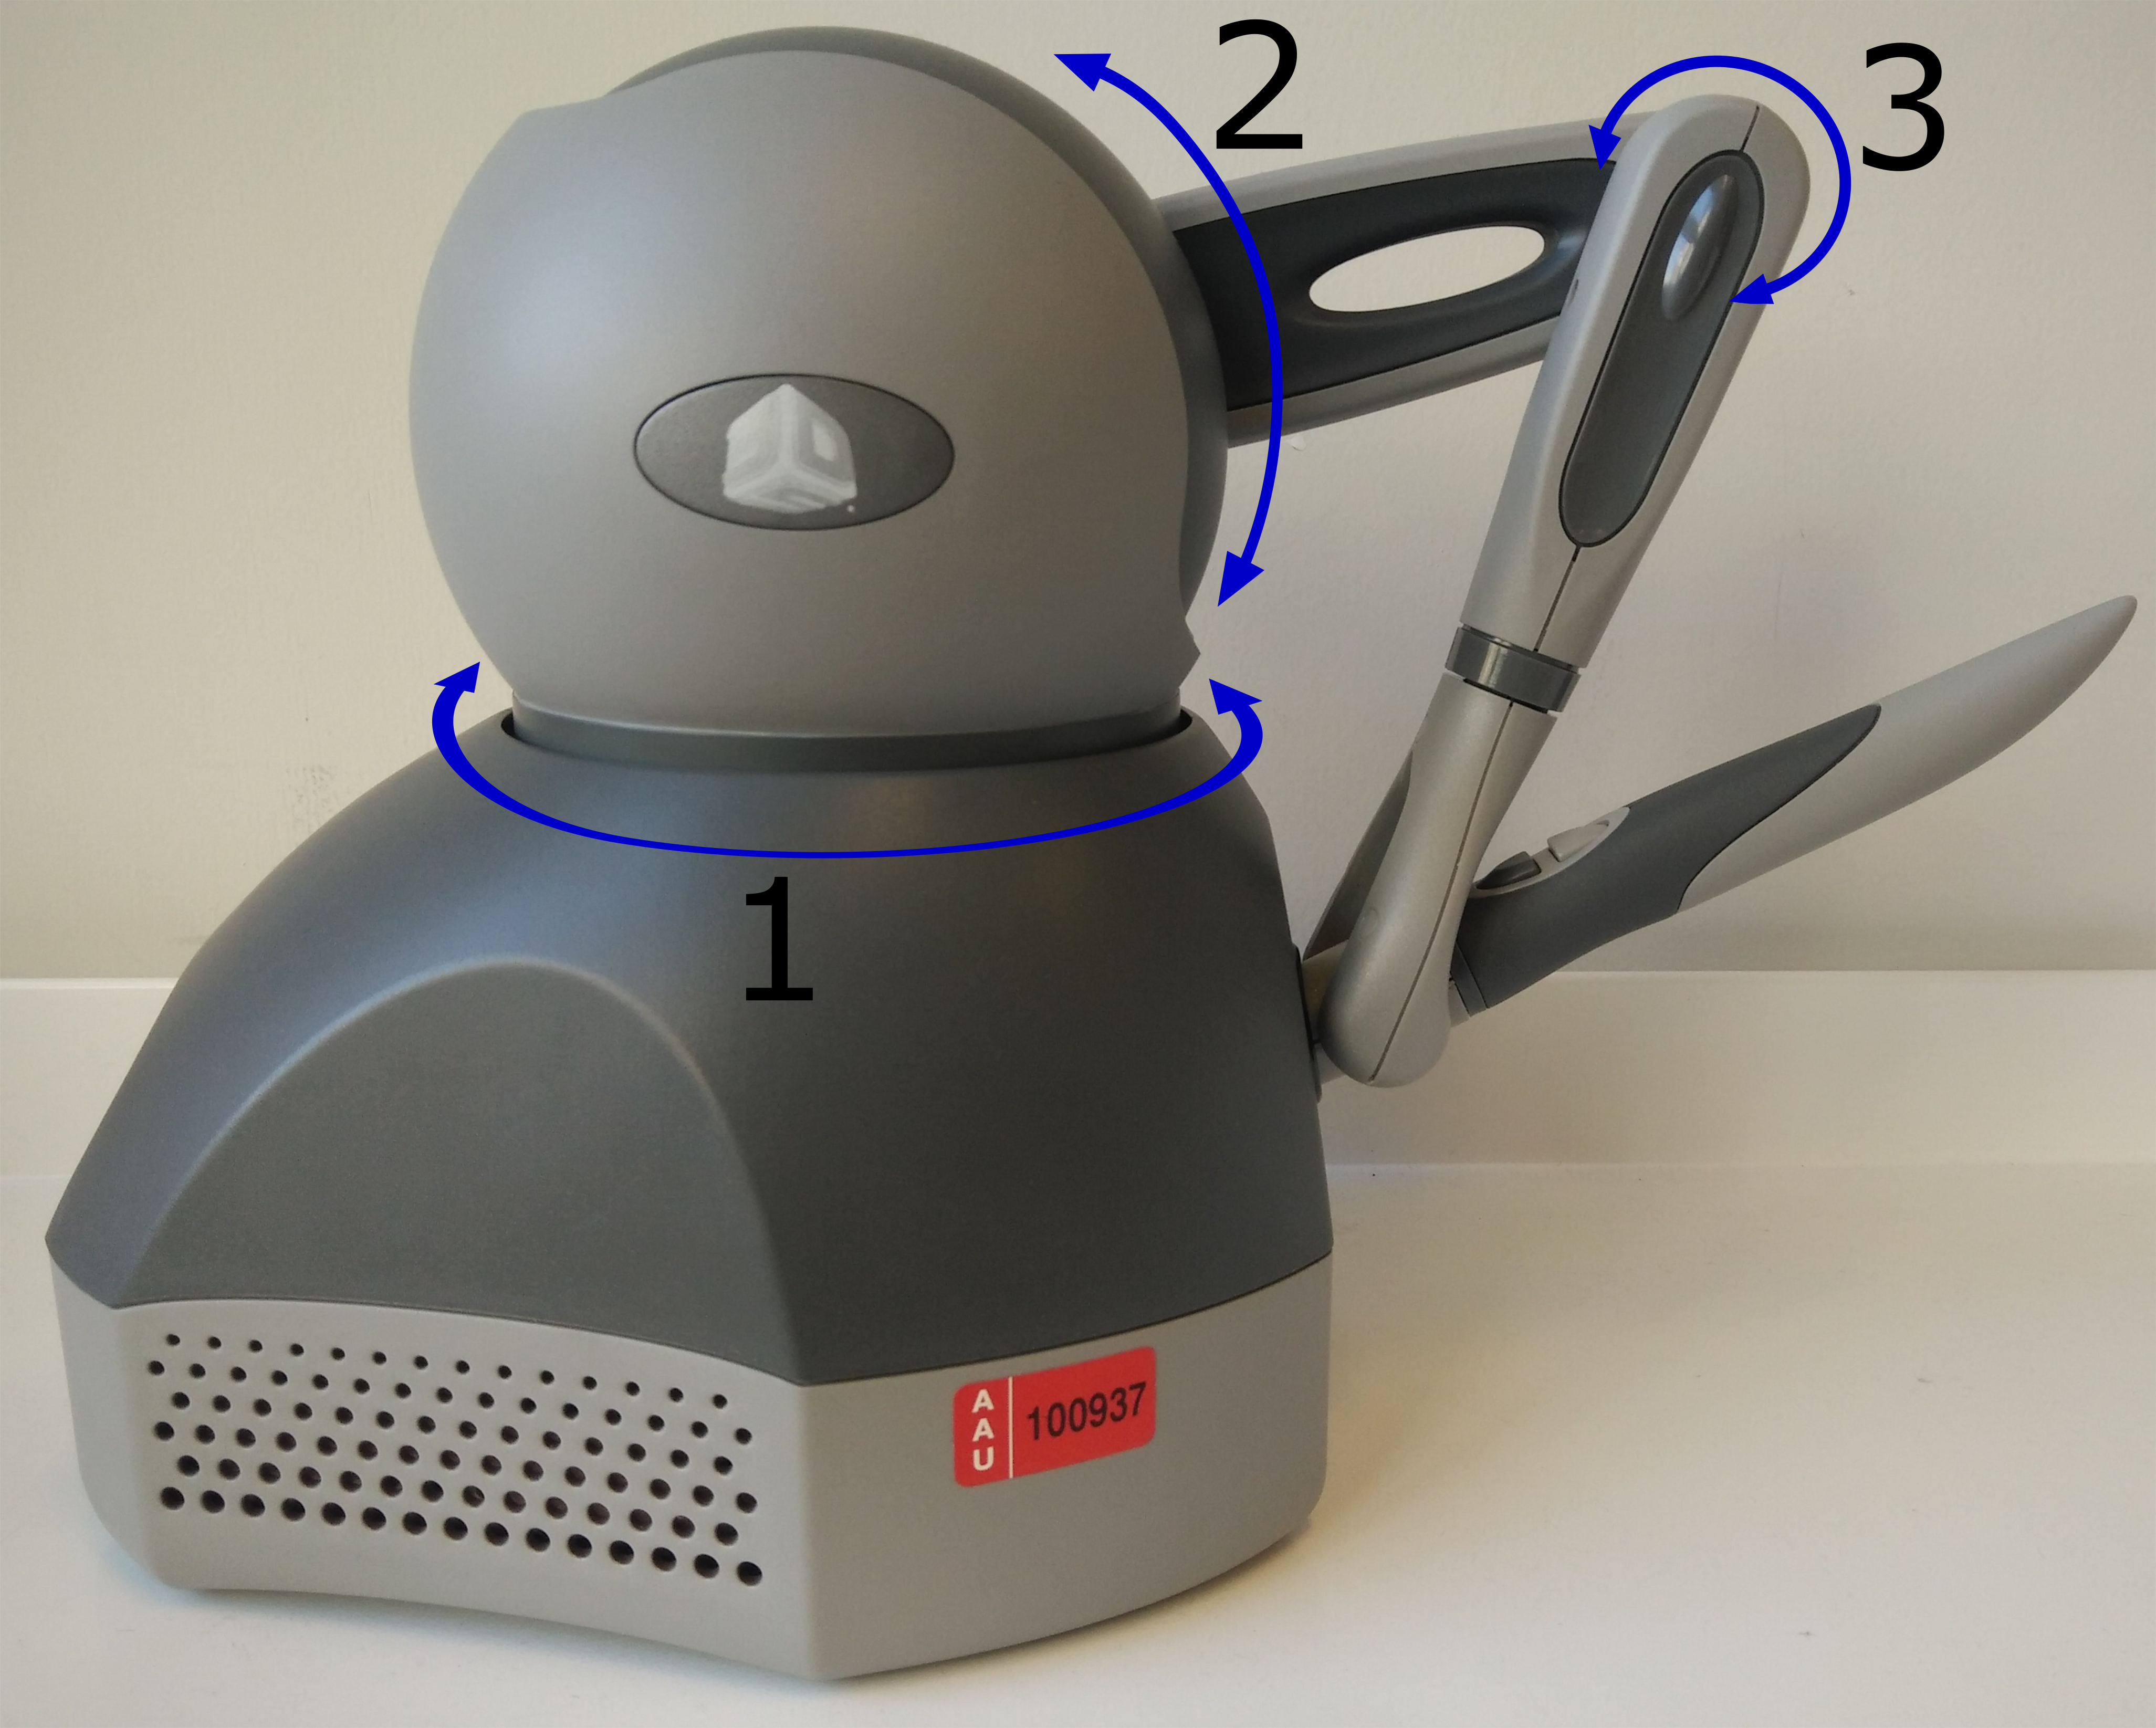
\includegraphics[width=\linewidth]{haptick1.jpg}
		\caption{Overview of the Phantom omni's first three joints.}
		\label{fig:phantom1}
	\end{subfigure}
	\begin{subfigure}{.45\textwidth}
		\centering
		\includegraphics[width=\linewidth]{haptick2.png}
		\caption{Overview of the Phantom omni's last three joint}
		\label{fig:phantom2}
	\end{subfigure}
\caption{Overview of all the Phantom omni's joints\citep{phantom_omni}}
\label{fig:phantom_omni}
\end{figure}

As mentioned the Phantom omni has the ability to generate resistance for the user. In other words, when moved in a specific direction it can create a counter force in respect to a certain position. On \figref{fig:phantom_omni}, it can be seen that the omni has six \gls{DOF}, where the first three has actuators. This means that the device only has the ability to generate force feedback with three \gls{DOF}, in this case roll, pitch and yaw.

The connection to the omni can either be made directly through a ethernet cabel or through ethernet cabel to a usb converter into a computer. For programming the omni an API is included, which enables the connection to the omni. The programming of the omni happens through the languages C++. \todo{include other languages}


% \begin{figure}[H]
% \centering
% \scalebox{1}{\input{rapport/pictures/phantom_omni.png}}
% \caption{Block diagram of the cascade.}
% \label{fig:RegBlock2}
% \end{figure}


\begin{figure}[H]
\centering
\begin{tikzpicture}
%\draw (-1.5,-1.5) rectangle (13.5,1.5);

\draw (-2.8,3.1) rectangle (2.8,-12.8);
\node at (0,2.5) {\textbf{sbRIO}};


\draw (-2.5,2) rectangle (2.5,-4.2);
\node at (0,1.5) {\textbf{Micro processor}};
\node[box] (datlog) at (0,0.3) {Data logging};
\node[box] (ethcommu) at ($(0,-1.7) + (datlog)$) {Ethernet communication};
\node[box] (shuterr) at ($(0,-1.7) + (ethcommu)$) {Shutdown:\\Communication error};


\draw (-2.5,-4.7) rectangle (2.5,-12.6);
\node at (0,-5.2) {\textbf{FPGA}};
\node[box] (poscon) at ($(0,-3.3) + (shuterr)$) {Position control};
\node[box] (enco) at ($(0,-1.7) + (poscon)$) {Encoder counter};
\node[box] (PWM) at ($(0,-1.7) + (enco)$) {PWM control};
\node[box] (dataES) at ($(0,-1.7) + (PWM)$) {Read data: ESCON};


\draw (-9,-6) rectangle (-4,-12.6);
\node[box] (spcon) at (-6.5,-8) {Speed control\\with inner current\\control};
\node at ($(spcon) + (0,1.5)$) {\textbf{ESCON}};
\node at ($(spcon) + (0,1.2)$) {\textbf{motor controller}};
\node[box] (limcu) at ($(0,-1.7) + (spcon)$) {Limit output\\current};
\node[box] (reen) at ($(0,-1.7) + (limcu)$) {Read encoder\\ticks};


\draw (-9,-5.5) rectangle (-4,-4);
\node at (-6.5,-4.75) {\textbf{Motor}};


\draw (-9,-3.5) rectangle (-4,3.1);
\node at (-6.5,2.5) {\textbf{ROS computer}};

%\node[fill = {rgb:red,1;green,2;blue,5},box] (Opt) at (0,0) {Operator};
%\node[fill = {rgb:red,1;green,2;blue,5},box] (Geo) at ($(3,0) + (Opt)$) {};
%\node[fill = {rgb:red,1;green,2;blue,5},box] (ros) at ($(3,0) + (Geo)$) {Robotic\\operating\\system};
%\node[fill = {rgb:red,1;green,2;blue,5},box] (davin) at ($(3,0) + (ros)$) {Da Vinci\\robot};
%\node[fill = {rgb:red,1;green,2;blue,5},box] (end) at ($(3,0) + (davin)$) {Endowrist};


%\draw[->, ultra thick] ([yshift=0.3cm]Opt.east) -- ([yshift=0.3cm]Geo.west);
%\draw[->, ultra thick] ([yshift=0.3cm]Geo.east) -- ([yshift=0.3cm]ros.west);
%\draw[->, ultra thick] ([yshift=0.3cm]ros.east) -- ([yshift=0.3cm]davin.west);
%\draw[->, ultra thick] ([yshift=0.3cm]davin.east) -- ([yshift=0.3cm]end.west);


%\draw[<-, ultra thick] ([yshift=-0.3cm]Opt.east) -- ([yshift=-0.3cm]Geo.west);
%\draw[<-, ultra thick] ([yshift=-0.3cm]Geo.east) -- ([yshift=-0.3cm]ros.west);
%\draw[<-, ultra thick] ([yshift=-0.3cm]ros.east) -- ([yshift=-0.3cm]davin.west);
%\draw[<-, ultra thick] ([yshift=-0.3cm]davin.east) -- ([yshift=-0.3cm]end.west);

%\node at (1.5,1) {Position};
% \node at (4.5,1) {Position};
% \node at (7.5,1) {yes};
% \node at (10.5,1) {yes};

%\node at (1.5,-1) {Force};
% \node at (4.5,1) {Position};
% \node at (7.5,1) {yes};
% \node at (10.5,1) {yes};
\end{tikzpicture}
\caption{Overall system with feedback in both direction}
\end{figure}




%\input{rapport/system_dis/communication_com.tex}

%\input{rapport/system_dis/Test_setup.tex}



\section{Endowrist}\label{sec:Endowrist}

An Endowrist, see \figref{fig:Endo_full} is a surgical tool which can be manipulated as a human wrist. It is used in surgical procedures such as Laparoscopic surgeries, better known as minimally invasive surgery (MIS), where small incisions in the human body is made under the surgery. Because the incision cuts are small, blood lose under the surgery and the risk of infection is reduced. This has a positive effect on the recovery time for the patient.


\begin{figure}[H]
	\centering
	\begin{subfigure}{.32\textwidth}
		\centering
		\includegraphics[width=\linewidth]{Endowrist1.jpg}
		\caption{Full view of a Endowrist\vspace{8.5mm}   }
		\label{fig:Endo_full}
	\end{subfigure}
	\begin{subfigure}{.32\textwidth}
		\centering
		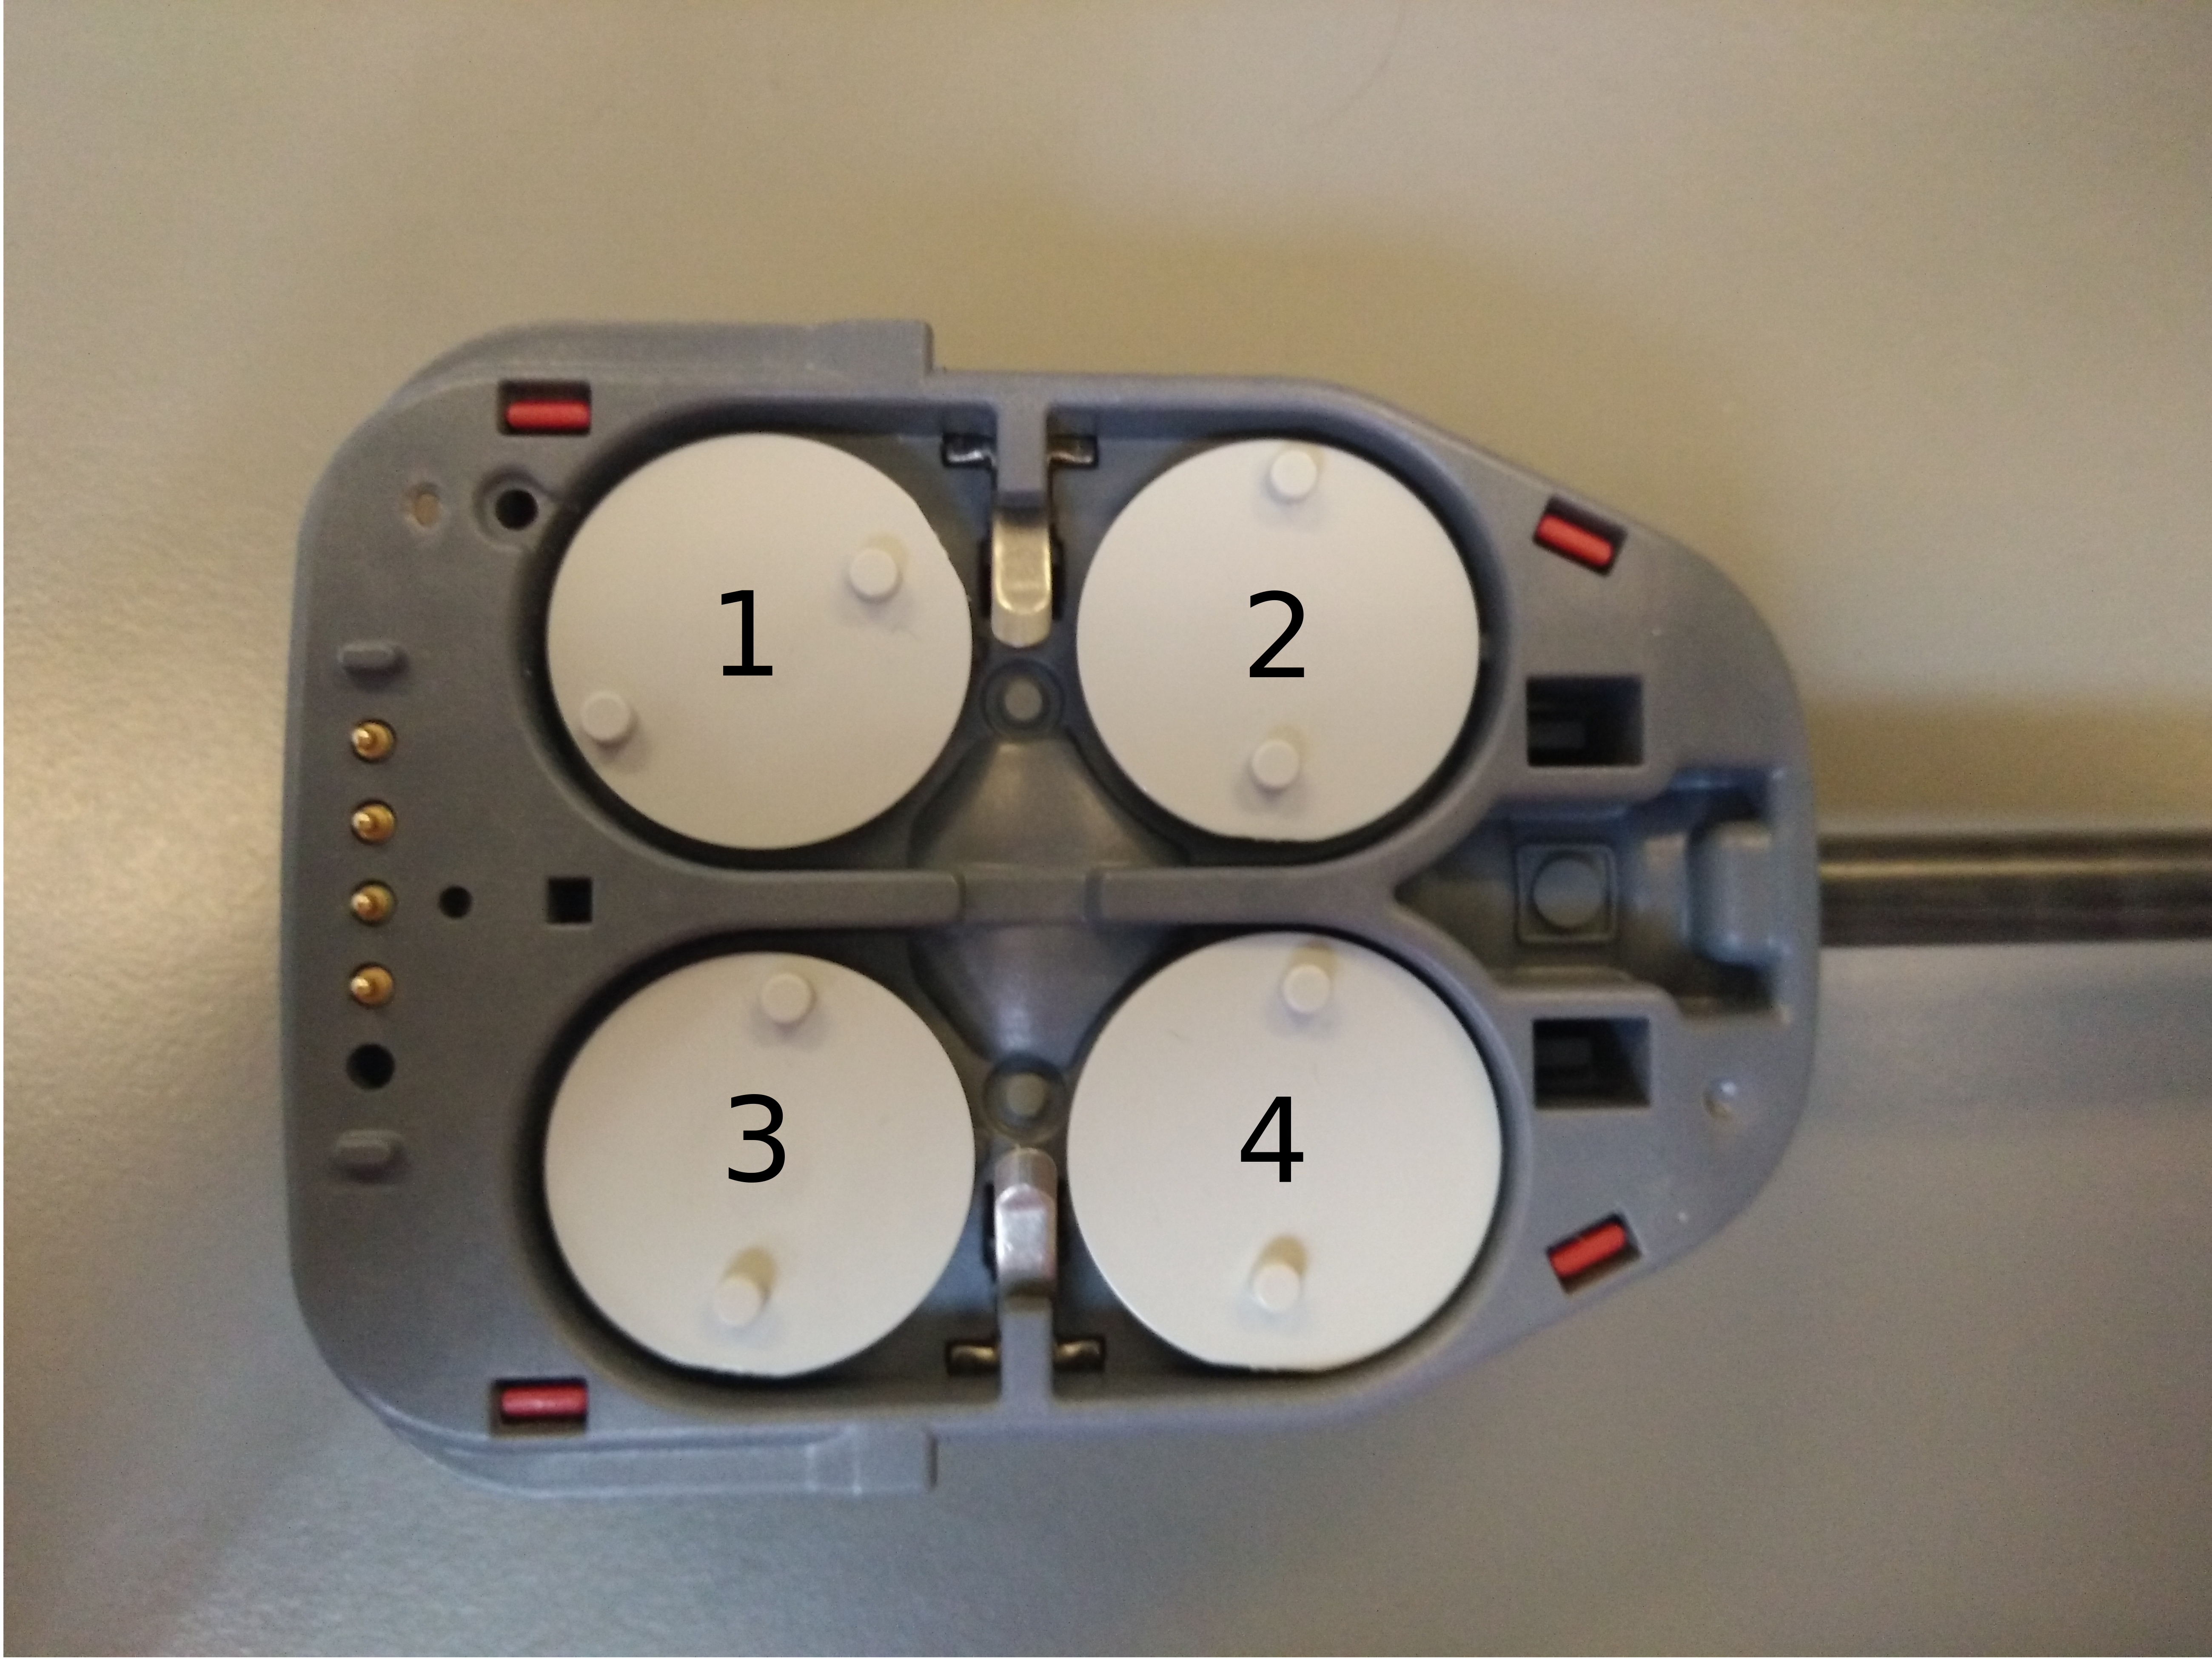
\includegraphics[width=\linewidth]{Endowrist2.jpg}
		\caption{Actuator plates, which can alternate the end effector position}
		\label{fig:Endo_plates}
	\end{subfigure}
	\begin{subfigure}{.32\textwidth}
		\centering
		\includegraphics[width=\linewidth]{Endowrist3.jpg}
		\caption{End effector of the Endowrist\newline}
		\label{fig:Endo_end}
	\end{subfigure}
\caption{The Endowrist and how the interaction with it are made}
\label{fig:endowrits_set}
\end{figure}

As mentioned the Endowrist has the ability to be manipulated as a human wrist and thereby has four \gls{DOF}, see \figref{fig:Endo_end}.\todo{We have to update the picture so it shows each DOF}. This enables the movement of roll, pitch, yaw and an open closing mechanism that acts as the thumb and index finger of a hand. 

The end effector is manipulated by the four wheels seen on \figref{fig:Endo_plates}\todo{update with numbers}. Wheel one and three defines the movement of the yaw and the closing mechanism. Wheel two moves the pitch and wheel four is for the roll. Each wheel drives a cable inside the Endowrist, which transport a force at one end to the other. The Endowrist is cable driven, which enables the opportunity of making the Endowrist small but it also makes the system nonlinear as the force acting at one end is not directly transmitted to the other end due to friction. 





%\subsection{ROS}\label{sec:ros}

In order to communicate between ROS and the sbRIO board the university created a ROS node called davinci\_driver. This driver is composed of three parts:

\begin{itemize}
\item Low level driver
\item Middel level driver
\item High level driver
\end{itemize}

The low level driver communicate directly with the sbRIO board. The high level driver handled the communication between ROS nodes. It updates the data for the nodes and transmits the setpoints to the low level driver through the middel driver. The name "setpoint" is used to designate the next position a motor should take.

The middle level driver handles the creation(s) of the low lever driver(s) and communication between the low and high level driver, so there is no need for the client to acquire mutexes. Due to the opportunity of creating more than one low lever driver it is possible to communicate with more than one arm of the DaVinci robot.\todor{Just this column of text}

The low level driver connects to one sbRIO board using a TCP/IP socket and launch a loop in a thread to handle the communication. The data exchange is made using \gls{JSON} files, see \secref{subsec:JSON}. The structure of the code can be seen in\figref{fig:original_driver}.

\begin{figure}[H]
\centering
\begin{tikzpicture}

\node[box] (Initialization) at (0,0) {Initialization};
\node[box] (Receive) at ($(0,-2)+(Initialization)$) {Read the data \\if some were received};
\node[box] (Send) at ($(0,-2)+(Receive)$) {Send if the\\ control changed};
\node[box] (Sleep) at ($(0,-2)+(Send)$) {Sleep};
\node[box] (Update_State) at ($(5,0)+(Receive)$) {Update the data\\ available for higher\\level processes};

\draw[->, ultra thick] (Initialization) -- (Receive);
\draw[->, ultra thick] (Receive) -- (Update_State);
\draw[->, ultra thick] (Receive) -- (Send);
\draw[->, ultra thick] (Send) -- (Sleep);
\draw[->, ultra thick] (Sleep.west) -| ++(-2,0) |- (Receive);

\end{tikzpicture}
\caption{Structure of the original sbRIO driver}
\label{fig:original_driver}
\end{figure}
\todo{Figure is still unclear, make 5 lines of text describing the flow}

% The middle level driver allows the creation of more than one low level driver. Due to this it is possible to communicate with more than one arm of the DaVinci Robot at once. It also handles the communication between the high level driver and the low level so that there is no need for the client to acquire mutexes.\todo{last sentence - half of it is double confetti}

\section{Electronics}\label{sec:electronics}
% Small introduction to tikz figures and its basics, can be found on 
% http://cremeronline.com/LaTeX/minimaltikz.pdf
% Under the file tikz_magic.tex all the different boxes can be found!
%\subsection{Single board reconfigurable I/O}

\todo{Sloth reference}
The electronic setup contains a \textbf{\textit{Single Board Reconfigurable Input/Output 9636}} (sbRIO) controller which is responsible for interfacing between the surgical robot and the computer running ROS\todo{maby ref to ROS section}. It reads the sensor measurements, sends them to the PC and controls the motors based on the received reference signals. The sbRIO has built in safety protocols that disable the motors in case of error.

The controller consists of
\begin{itemize}
	\item 400 MHz real time processor
	\item 256 MB of system memory and 512 MB nonvolatile memory
	\item Reconfigurable Xilinx Spartan-6 LX45 FPGA
	\item 16 bit analog and digital I/O
	\item Built in USB, CAN, 10/100 Mb/s Ethernet peripherials
\end{itemize}

The board is configured through ethernet cable. The programs can be written in Labview, C or C++. We used LabView code to operate the sbRIO. The board is capable of running Real-time. %code, which is unmatched on the ROS side.

% http://sine.ni.com/nips/cds/view/p/lang/en/nid/210421

\subsection{Hardware setup}

The Endowrists, see \figref{fig:endowrits_set}, is actuated by 4 Maxon DC motors, see \secref{Maxon_Motor}. Each motor is equipped with an ESCON motor controller responsible for the cascade speed and inner loop current control. The control reference is sent through the sbRIO. They also provide current measurements to the sbRIO. Each motor hosts an encoder and a potmeter that provide absolute and relative angular position information to the FPGA built into the sbRIO board. For an graphical illustration of the connection see \figref{electro_setup}.
 
\todo{Complete the diagram}
\todo{som explanation for the next line UDP, or erase it?}
The sbRIO communicates with the PC using UDP protocol. 
\input{rapport/system_dis/Eletronic_component.tex}

\todo{elaborate this picture, what do the different boxes do?}


\subsection{Motor}\label{Maxon_Motor}
The four motors for actuating the Endowrist is sold as a bulk solution which include motor\cite{motor_motor}, gear\cite{motor_gear} and a position encoder\cite{motor_encoder}, see \figref{fig:Full_motor _dis}.

The control of these motors are done through the ESCON motor drivers, which are connected to the sbRIO board.\todo{ESCON motor driver needed!}

%The ESCON motor controllers are attached to the sbRIO controller and send the control signals through cables. The motor has a nominal torque of 6.96 mNm.
%4 Maxon motors are used for the actuation of the endowrist. The motors are implemented using a combination gear (Maxon 353816) including the gearing, the servo motor and the sensors. The ESCON motor controllers are attached to the sbRIO controller and send the control signals through cables. The motor has a nominal torque of 6.96 mNm.

\begin{figure}[H]
	\centering
	\begin{subfigure}{.32\textwidth}
		\vspace{0pt}
		\centering
		\includegraphics[width=\linewidth]{motor.jpg}
		\caption{The Maxon 110160 \newline DC motor}
		\label{fig:motor}
	\end{subfigure}
	\begin{subfigure}{.32\textwidth}
		\centering
		\includegraphics[width=\linewidth]{motor_gear.jpg}
		\caption{The planetary gearhead equipped with sleeve bearing}
		\label{fig:motor_gear}
	\end{subfigure}
	\begin{subfigure}{.32\textwidth}
		\centering
		\includegraphics[width=\linewidth]{motor_sensor.jpg}
		\caption{The encoder used for getting angular data}
		\label{fig:motor_sensor}
	\end{subfigure}
	\caption{The combination gear disassembled}
	\label{fig:Full_motor _dis}
\end{figure}



\section{Overview}
\todor{This section has to be read}
As mentioned before, a fully featured DaVinci robot has four arms with 6-7 \gls{DOF} in total, when the Endowrist instrument included.
%Since the robot has 4 arms, there are 4 instruments.
%Although our setup controls only 4 motors, in funcionality it is equivalent to one DaVinci arm.
Although our setup controls only 4 motors, which gives the fully functionalities of manipulating one surgical tool.

The sbRio board controls the test setup and as such represents the onboard computer on the DaVinci robot.
In order to perform higher level functions such as force feedback control, it is necessary to remotely handle data and send high-level commands.
This is handled by an external computer system that is connected to the Geo magic touch device.

The sbRio board communicates with the computer using UDP communication protocols, while the Geomagic touch does so using TCP/IP.
The computer also performs force estimation using a dynamical model of the test setup (or Endowrist, more precisely), this is vital for force feedback.
In order to connect software components responsible for communicating with hardware and the ones responsible for the control algorithm and estimation.
For this purpose we use the Robot Operating System (ROS), which uses a network architecture to share data between components via data streams.

\begin{figure}
\begin{tikzpicture}
\draw (-1.5,-1.5) rectangle (13.5,1.5);


\node[fill = {rgb:red,1;green,2;blue,5},box] (Opt) at (0,0) {Operator};
\node[fill = {rgb:red,1;green,2;blue,5},box] (Geo) at ($(3,0) + (Opt)$) {Geomagic\\touch};
\node[fill = {rgb:red,1;green,2;blue,5},box] (ros) at ($(3,0) + (Geo)$) {Robotic\\operating\\system};
\node[fill = {rgb:red,1;green,2;blue,5},box] (davin) at ($(3,0) + (ros)$) {Da Vinci\\robot};
\node[fill = {rgb:red,1;green,2;blue,5},box] (end) at ($(3,0) + (davin)$) {Endowrist};


\draw[->, ultra thick] ([yshift=0.3cm]Opt.east) -- ([yshift=0.3cm]Geo.west);
\draw[->, ultra thick] ([yshift=0.3cm]Geo.east) -- ([yshift=0.3cm]ros.west);
\draw[->, ultra thick] ([yshift=0.3cm]ros.east) -- ([yshift=0.3cm]davin.west);
\draw[->, ultra thick] ([yshift=0.3cm]davin.east) -- ([yshift=0.3cm]end.west);


\draw[<-, ultra thick] ([yshift=-0.3cm]Opt.east) -- ([yshift=-0.3cm]Geo.west);
\draw[<-, ultra thick] ([yshift=-0.3cm]Geo.east) -- ([yshift=-0.3cm]ros.west);
\draw[<-, ultra thick] ([yshift=-0.3cm]ros.east) -- ([yshift=-0.3cm]davin.west);
\draw[<-, ultra thick] ([yshift=-0.3cm]davin.east) -- ([yshift=-0.3cm]end.west);

\node at (1.5,1) {Position};
% \node at (4.5,1) {Position};
% \node at (7.5,1) {yes};
% \node at (10.5,1) {yes};

\node at (1.5,-1) {Force};
% \node at (4.5,1) {Position};
% \node at (7.5,1) {yes};
% \node at (10.5,1) {yes};
\end{tikzpicture}
\caption{Overall system with feedback in both direction}
\end{figure}






